% CVPR 2026 Paper Template; see https://github.com/cvpr-org/author-kit

\documentclass[10pt,twocolumn,letterpaper]{article}

%%%%%%%%% PAPER TYPE  - PLEASE UPDATE FOR FINAL VERSION
\usepackage{cvpr}              % To produce the CAMERA-READY version

\usepackage{microtype}
% XeLaTeX cannot load the template's `times' fonts and falls back to the wider Latin Modern, which changes the page
% count; use the equivalent TeX Gyre Termes there so pdflatex and xelatex give the same layout.
\usepackage{iftex}
\ifXeTeX
  \usepackage{fontspec}
  \setmainfont{TeX Gyre Termes}
\fi
\usepackage{multirow}

\definecolor{cvprblue}{rgb}{0.21,0.49,0.74}
\usepackage[pagebackref,breaklinks,colorlinks,allcolors=cvprblue]{hyperref}

%%%%%%%%% PAPER ID  - PLEASE UPDATE
\def\paperID{*****} % *** Enter the Paper ID here
\def\confName{CVPR}
\def\confYear{2026}

\newcommand{\pmstd}[1]{{\scriptsize$\pm$#1}}
\newcommand{\code}[1]{\texttt{\small #1}}

%%%%%%%%% TITLE - PLEASE UPDATE
\title{Assignment 1: Self-Supervised Learning with SimSiam on STL-10}

%%%%%%%%% AUTHORS - PLEASE UPDATE
\author{B12508026 TAI, WEI-HSUAN}

\begin{document}
\maketitle

%%%%%%%%% ABSTRACT
\begin{abstract}
We re-implement SimSiam~\cite{chen2021simsiam} with ResNet-18 on the 100k unlabeled STL-10 images.
With 1,000 labels, a linear probe on the frozen encoder reaches $80.98\pm0.35\%$ test accuracy (200 epochs, 3 seeds), versus $55.66\pm0.93\%$ for a tuned from-scratch network.
Removing the stop-gradient or the predictor reproduces the paper's complete collapse (exactly 10.00\%, chance).
As a new ablation, we remove one augmentation family at a time. Without cropping, SimSiam suffers \emph{dimensional collapse} (backbone effective rank 6.7 vs.\ 318), and rank and accuracy \emph{drop} with longer training.
Replacing the crop shows that the views must \emph{differ}: one crop shared by both views is as bad as none, random masking recovers two thirds of the gap, and permuted tiles barely help. Each model becomes invariant mainly to what its views differ by, and the crop's part-to-whole rescaling classifies best.
\end{abstract}

%%%%%%%%% BODY TEXT
\section{Introduction}
\label{sec:intro}

SimSiam~\cite{chen2021simsiam} trains a Siamese network to make the representations of two augmented views of an image agree, with no negative pairs, large batches or momentum encoder.
Contrastive methods such as SimCLR~\cite{chen2020simclr} rely on negatives to avoid the constant solution, BYOL~\cite{grill2020byol} on a momentum encoder; SimSiam claims that a stop-gradient and a predictor alone suffice.

Without negatives, the difference between the two augmented views is SimSiam's \emph{only} learning signal.
SimCLR~\cite{chen2020simclr} found crop plus color the most important augmentation pair for contrastive learning, and InfoMin~\cite{tian2020infomin} argues that good views should share task-relevant information and differ in everything else.
The SimSiam paper, however, ablates the architecture and the loss but not the augmentations that create this signal; BYOL~\cite{grill2020byol} removed augmentations but did not analyze the representations.
We re-implement SimSiam on STL-10~\cite{coates2011stl10} and study both.
We (i) show that pretraining beats a tuned from-scratch baseline by 25.3 points with 1,000 labels (\cref{sec:exp_cls}); (ii) reproduce the collapse without stop-gradient or predictor (\cref{sec:exp_arch}); (iii) find \emph{dimensional collapse} without cropping that worsens with training (\cref{sec:exp_aug}); and (iv) decompose the crop: the views must differ in content, and each model learns mainly the invariance its views demand (\cref{sec:exp_crop}).

%-------------------------------------------------------------------------
\section{Environment and Codebase}
\label{sec:env}

All experiments ran on one NVIDIA GeForce RTX 5070 Ti (16\,GB, driver 570.211.01, CUDA 12.8) with Python 3.10.21, PyTorch 2.8.0, torchvision 0.23.0 and cuDNN 9.10.2 (\cref{fig:env}).
The code extends the course starter code.
\code{model.py} holds SimSiam and its loss, with \code{stop\_grad} and \code{predictor} flags for the ablations; \code{data.py} the STL-10 loaders, validation split and two-view augmentation with an \code{aug} option (\cref{sec:method});
\code{pretrain.py} logs loss, kNN accuracy and output std every epoch; \code{linear\_probe.py} trains a linear (or BN) probe on the frozen backbone and \code{sft.py} the same ResNet-18 from scratch.
\code{analyze\_*.py}, \code{eval\_probes.py} and \code{stats\_tests.py} compute erank, AUROC/F1, invariance and tests; \code{run\_*.sh} drive all experiments.

\begin{figure}[t]
\centering
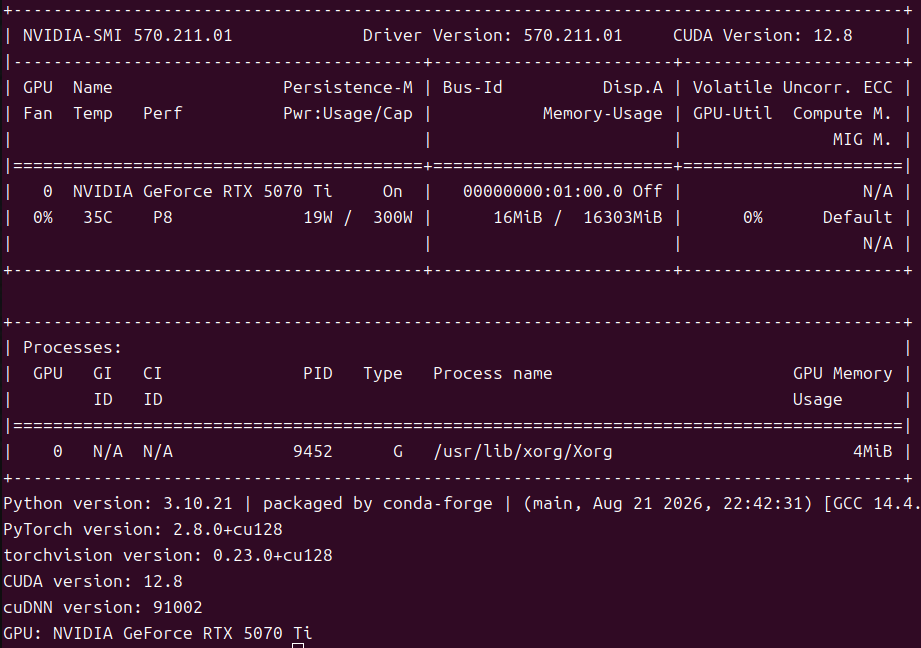
\includegraphics[width=0.82\linewidth]{figures/screenshot_cropped.png}
\caption{Experimental environment}
\label{fig:env}
\end{figure}

%-------------------------------------------------------------------------
\section{Method}
\label{sec:method}

\subsection{SimSiam}
Given an image $x$, two random augmentations produce views $x_1$ and $x_2$.
An encoder $f$, consisting of a backbone and a projection MLP, maps each view to $z_i=f(x_i)$, and a prediction MLP $h$ maps it to $p_i=h(z_i)$.
With the negative cosine similarity $\mathcal{D}(p,z)=-\frac{p}{\|p\|_2}\cdot\frac{z}{\|z\|_2}$, the symmetric loss is
\begin{equation}
\mathcal{L}=\tfrac12\mathcal{D}(p_1,\text{sg}(z_2))+\tfrac12\mathcal{D}(p_2,\text{sg}(z_1)),
\label{eq:loss}
\end{equation}
where $\text{sg}(\cdot)$ is the stop-gradient. The minimum of $\mathcal{L}$ is $-1$.

We use a ResNet-18 backbone~\cite{he2016resnet} with its fc layer removed (512-d output), a 3-layer projection MLP ($512\!\to\!2048\!\to\!2048\!\to\!2048$, BN~\cite{ioffe2015bn} on every layer) and a bottleneck prediction MLP ($2048\!\to\!512\!\to\!2048$).

\subsection{Ablations}
\paragraph{Architecture.}
Following Sec.~4.1--4.2 of the original paper, we (a) remove the stop-gradient so that gradients flow through both branches, and (b) replace the predictor $h$ with the identity.

\paragraph{Augmentation.}
The original paper's EM-like hypothesis (Sec.~5) views SimSiam as approximately solving
\begin{equation}
\min_\theta\; \mathbb{E}_{x,\mathcal{T}}\bigl\|f_\theta(\mathcal{T}(x))-\eta_x\bigr\|^2,
\label{eq:em}
\end{equation}
where $\eta_x$, optimized jointly with the encoder $f_\theta$, is at its optimum the mean representation of $x$ over augmentations $\mathcal{T}$.
If the augmentations are too weak, every $f_\theta$ nearly matches $\eta_x$, and Eq.~\eqref{eq:em} gives little signal.
To test this, we remove one family of augmentations at a time:
\textbf{no\_color} drops color jitter and grayscale, and \textbf{no\_crop} drops RandomResizedCrop, so that both views show the full image and differ only in flip and color.

\paragraph{Decomposing the crop.}
A crop shows only \emph{part} of the content, \emph{rescales and shifts} it, makes the two views differ and adds diversity across epochs. To separate these factors we replace it (keeping flip and color) with:
\textbf{crop\_in\_place} keeps a RandomResizedCrop-style region at its original position and scale and fills the rest with the ImageNet normalization mean (0 after normalization; partial content only);
\textbf{zoom\_out} shrinks the whole image to area fraction $a$ (crop-like aspect ratio) and pastes it at a random position on a mean-filled canvas (rescaling and shifting only);
\textbf{mask} keeps a random fraction $a$ of the 36 $16\!\times\!16$ patches and fills the rest with the mean (partial content, scattered, no rescaling);
\textbf{same\_crop} applies one random crop to \emph{both} views, so the data diversity matches the baseline but the views no longer differ in crop;
\textbf{shuffle} cuts each view into $2\!\times\!2$ tiles and permutes them independently (same content, different layout), and \textbf{shuffle\_shared} uses one permutation for both views (same seams, no layout difference) as its control.
In crop\_in\_place, zoom\_out and mask, $a\sim U(0.2,1)$ as in the crop, drawn independently for each view.

\begin{figure*}[t]
\centering
\begin{minipage}{0.495\linewidth}\centering
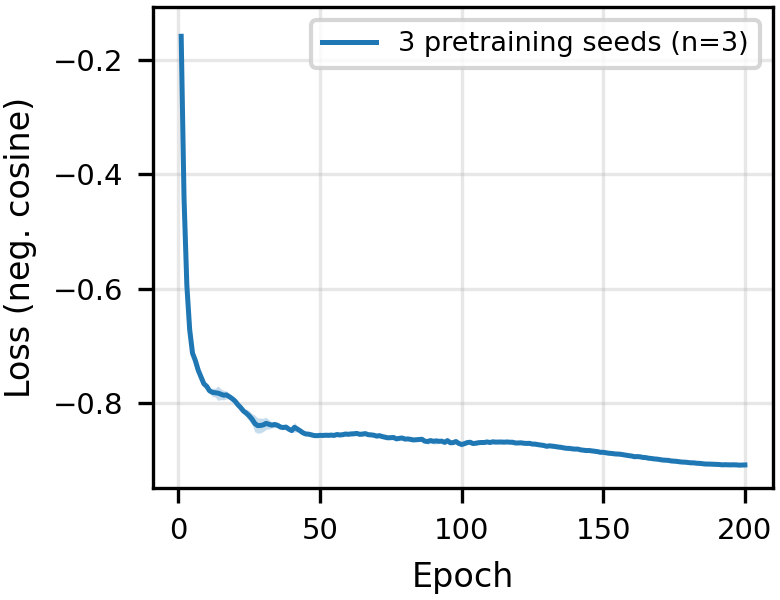
\includegraphics[width=0.49\linewidth]{figures/main_pretrain_loss.png}\hfill
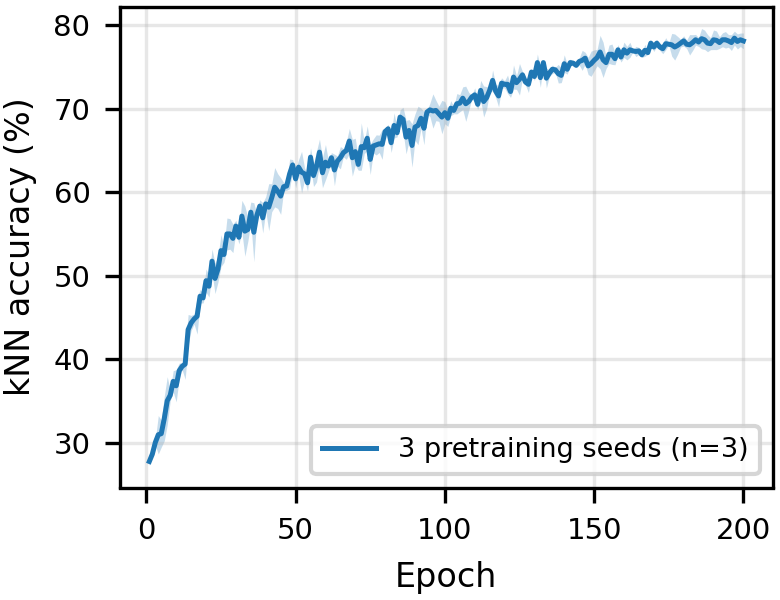
\includegraphics[width=0.49\linewidth]{figures/main_pretrain_knn.png}
\caption{SimSiam pretraining for 200 epochs, mean $\pm$ std over 3 pretraining seeds: training loss (left) and kNN validation accuracy (right).}
\label{fig:pretrain}
\end{minipage}\hfill
\begin{minipage}{0.495\linewidth}\centering
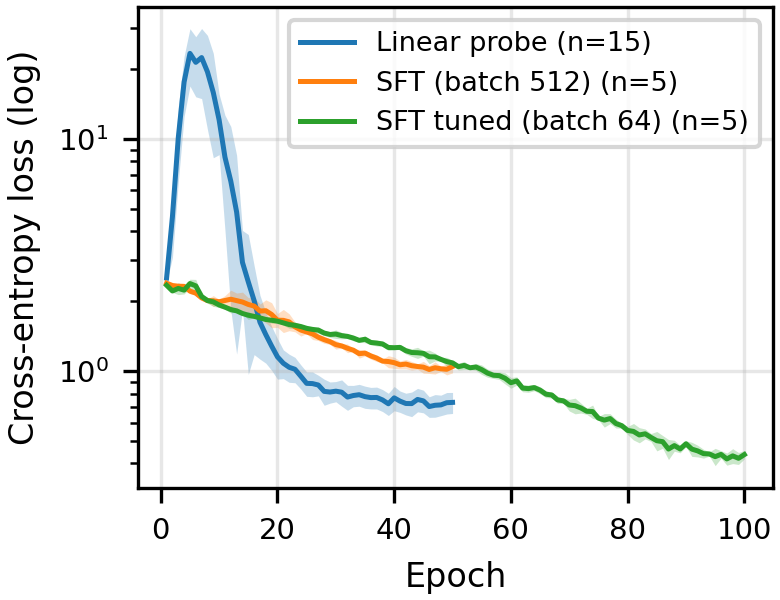
\includegraphics[width=0.49\linewidth]{figures/main_classify_loss.png}\hfill
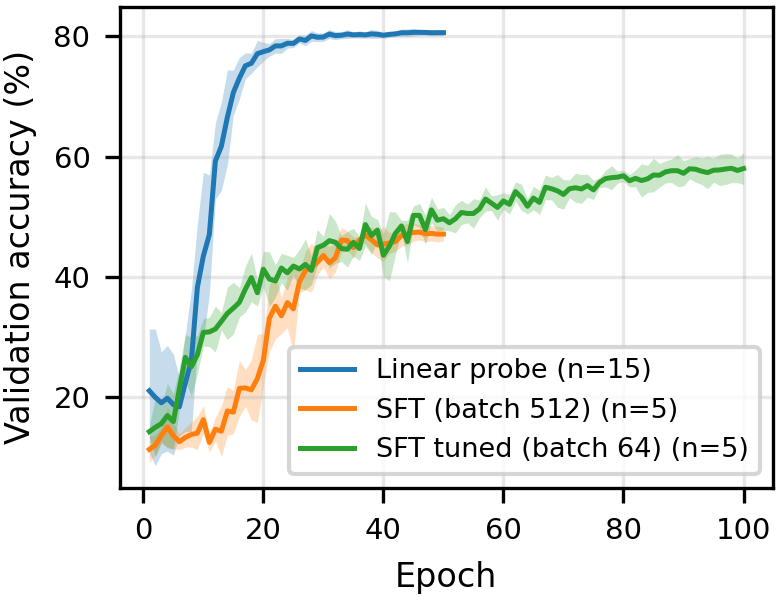
\includegraphics[width=0.49\linewidth]{figures/main_classify_val_acc.png}
\caption{Linear probe on frozen 200-epoch encoders (15 runs) vs.\ default and tuned SFT (5 runs each), mean $\pm$ std: training loss (left, log scale) and validation accuracy (right).}
\label{fig:cls}
\end{minipage}
\end{figure*}

\subsection{Measuring Collapse}
\emph{Complete collapse} maps every input to one vector; in \emph{dimensional collapse}~\cite{hua2021feature,jing2022dimensional} the embeddings stay spread out but occupy a low-dimensional subspace.
The std of the $\ell_2$-normalized output ($1/\sqrt{d}$ if spread, $0$ if collapsed) detects only the former, so we also measure the effective rank (erank)~\cite{roy2007erank}, which predicts downstream performance~\cite{garrido2023rankme}.
With $\sigma_k$ the singular values of the centered, $\ell_2$-normalized features of the 8,000 test images,
\begin{equation}
\text{erank}=\exp\Bigl(-\sum_k p_k\log p_k\Bigr),\quad p_k=\frac{\sigma_k}{\sum_j\sigma_j}.
\end{equation}
We focus on the 512-d backbone feature, the probe's input.

%-------------------------------------------------------------------------
\section{Experimental Setup}
\label{sec:setup}

\paragraph{Dataset.}
We use STL-10~\cite{coates2011stl10} at $96\times96$. Pretraining uses the 100k unlabeled images.
Classifiers train on the official fold~0 (1,000 images). Validation uses 500 held-out, label-balanced training images, and testing uses all 8,000 test images.

\paragraph{Pretraining.}
Following the original paper's CIFAR setting, we use SGD (momentum 0.9, weight decay $5\!\times\!10^{-4}$), batch size 512, $\text{lr}=0.03\times512/256$, a 10-epoch warmup and cosine decay. The augmentation is RandomResizedCrop (scale 0.2--1), horizontal flip, color jitter $(0.4,0.4,0.4,0.1)$ with $p{=}0.8$, and grayscale with $p{=}0.2$, without the Gaussian blur of its ImageNet setting. As in the paper, the predictor's lr is not decayed.
A kNN monitor~\cite{wu2018instance} ($k{=}200$, $\tau{=}0.1$) uses fold~0 as the memory bank and evaluates on the validation images after every epoch.

\paragraph{Evaluation.}
The \emph{linear probe} trains a linear layer on the frozen backbone with SGD (lr 30 as in MoCo~\cite{he2020moco}, no weight decay) for 50 epochs. The \emph{BN probe} adds a parameter-free BN before the linear layer as in MAE~\cite{he2022mae}, with lr chosen on validation.
The from-scratch baseline (\emph{SFT}) trains the whole ResNet-18 with the pretraining optimizer settings (batch 512, about 2 steps per epoch) for 50 epochs; a \emph{tuned SFT} uses batch 64 for 100 epochs with lr chosen on validation.
All classifiers (probes and SFT) train with RandomResizedCrop (scale 0.08--1) and horizontal flip.
The pretrained encoder is always the final-epoch checkpoint; for the classifier we test the \emph{probe/SFT epoch} with the best validation accuracy.

\paragraph{Statistics.}
For the 200-epoch comparisons we pretrain with seeds 123/456/789, and linear-probe each model with 5 finetuning seeds (12/34/56/78/90).
The \emph{pretraining seed} is the unit of replication: we report the mean $\pm$ std over the 3 per-model means and compare settings with two-sided Welch $t$-tests~\cite{welch1947}.
We also compute macro one-vs-rest AUROC and macro F1 for every probe, and check every comparison under all three metrics with Holm correction~\cite{holm1979} (one family of 25 tests per metric).

%-------------------------------------------------------------------------
\section{Experiments}
\label{sec:exp}

The original paper uses ImageNet and ResNet-50, so we compare only qualitative trends.


\subsection{SimSiam Pretraining}
\label{sec:exp_pretrain}



\Cref{fig:pretrain} shows 200-epoch pretraining over three seeds.
The loss falls to about $-0.77$ during the 10-epoch warmup and ends at $-0.908$ (all seeds within 0.001); the kNN accuracy rises steadily to 78.1\% (77.4--79.2).
The std of the normalized projector output ends at $0.0204$, close to $1/\sqrt{2048}=0.0221$, so the model has not collapsed.
From epoch 50 to 100 the loss moves by only 0.016 while kNN accuracy climbs from 61.6\% to 69.5\%.

\subsection{Classification with and without Pretraining}
\label{sec:exp_cls}



\begin{table}[t]
\centering
\small
\setlength\tabcolsep{4pt}
\begin{tabular}{lccc}
\toprule
Method & Pretrain & Test acc.\ (\%) & $n$ \\
\midrule
SFT from scratch & -- & 47.74\pmstd{1.17} & 5 ft.\ seeds \\
SFT, tuned$^\ddagger$ & -- & 55.66\pmstd{0.93} & 5 ft.\ seeds \\
Linear probe & 100 ep & 75.52 & 2 runs$^\S$ \\
Linear probe & 200 ep & \textbf{80.98}\pmstd{0.35} & 3 pt.\ seeds \\
Linear probe & 1000 ep & 86.74\pmstd{0.23} & 1 run$^\dagger$ \\
\bottomrule
\end{tabular}
\caption{Test accuracy with 1,000 labeled images. $^\dagger$One pretraining run, so $\pm$ covers finetuning seeds only. $^\S$Two unseeded runs (75.24, 75.80). $^\ddagger$Batch 64, 100 epochs, base lr (scaled by 64/256) picked on validation from $\{0.03,0.1,0.3\}$; 0.03 and 0.1 were run with one seed.}
\label{tab:cls}
\end{table}

Both classifiers use the same ResNet-18 and the same 1,000 labeled images (\cref{fig:cls}, \cref{tab:cls}).
The linear probe passes 70\% validation accuracy by epoch 15 and plateaus at 80.6\%; SFT stays near chance for 9 epochs and plateaus near 47\%, and tuned SFT reaches only 58\% after 100 epochs.
After 200 epochs of pretraining, the linear probe beats SFT by 33.2 points, and still by \textbf{25.3 points} (95\% CI 24.2--26.5, Welch $p{=}10^{-8}$; probe replicates are pretraining seeds, SFT replicates finetuning seeds) when SFT uses batch 64 (16 steps per epoch) and an lr tuned on validation.

Longer classifier training does not close the gap: SFT at batch 512 saturates at 49--50\% after 200 epochs (training loss 0.24), and a 200-epoch probe gains only $+0.8$.
Longer pretraining helps with diminishing returns (75.5, 81.0, 86.7\% after 100, 200, 1000 epochs), as in Tab.~4 of the original paper.

\begin{figure}[t]
\centering
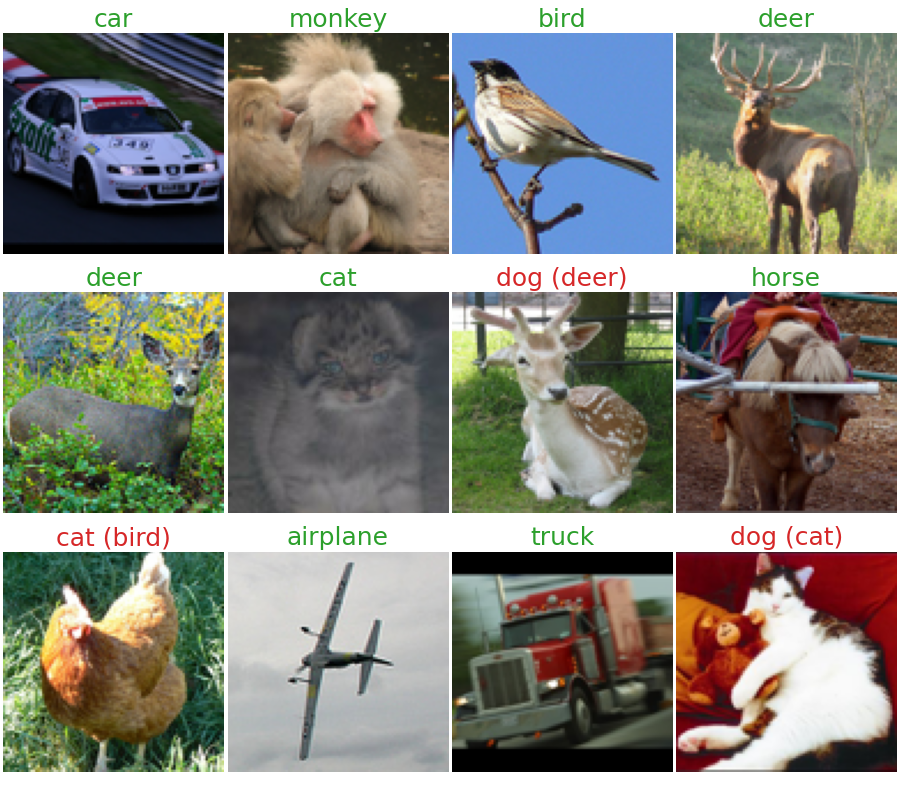
\includegraphics[width=0.5\linewidth]{figures/main_predictions.png}\hfill
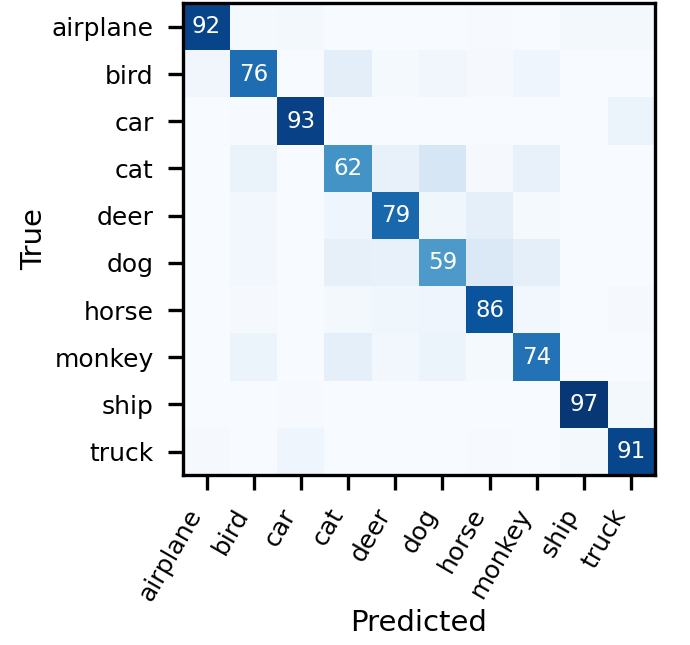
\includegraphics[width=0.44\linewidth]{figures/main_confusion.png}
\caption{Linear probe on the 200-epoch encoder: random test images, seed 123 (left; green correct, red ``prediction (truth)''), and the row-normalized confusion matrix pooled over 15 probes (right; diagonal: per-class accuracy, \%).}
\label{fig:pred}
\end{figure}

\paragraph{Error analysis.}
Errors are mostly between similar animals (\cref{fig:pred}): 16\% of cats are called dogs and 14\% of dogs horses, so cat and dog score lowest (62\%, 59\%) and vehicles highest (91--97\%).

\subsection{Ablation: Stop-Gradient and Predictor}
\label{sec:exp_arch}

\begin{figure*}[t]
\centering
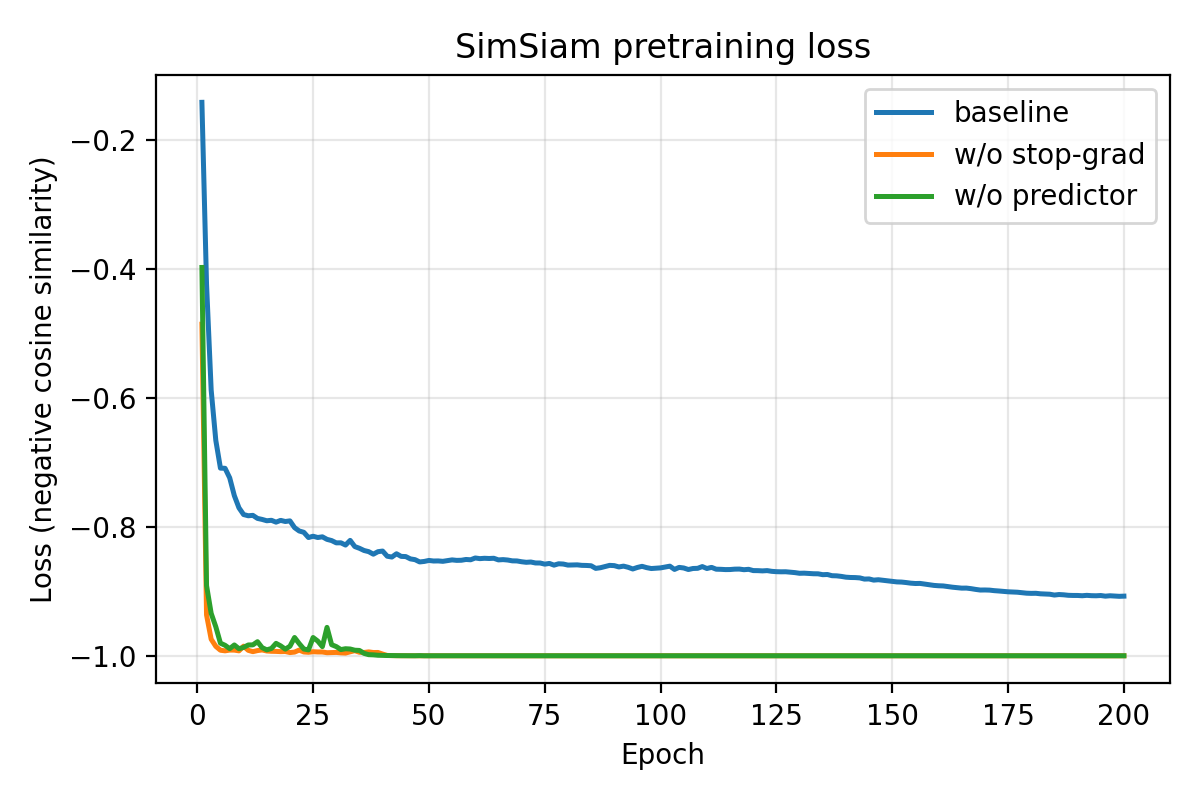
\includegraphics[width=0.325\linewidth]{figures/e200_arch_pretrain_loss.png}\hfill
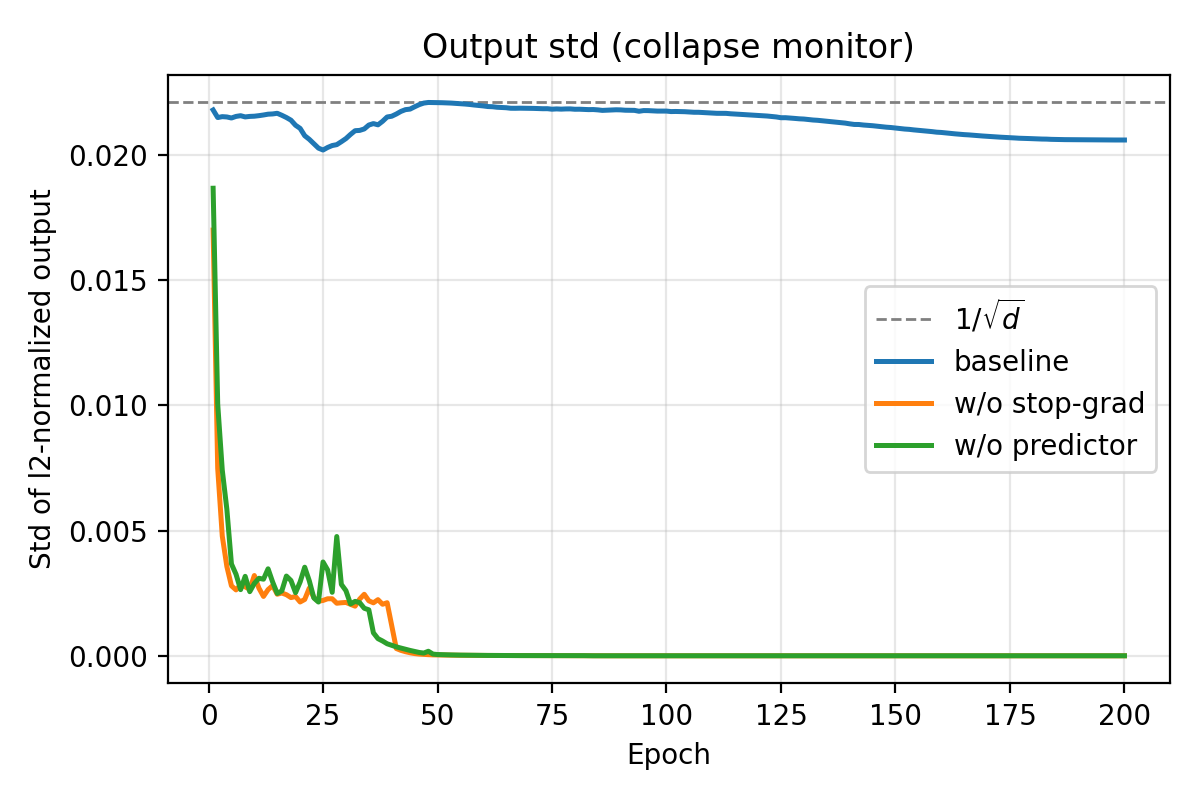
\includegraphics[width=0.325\linewidth]{figures/e200_arch_pretrain_std.png}\hfill
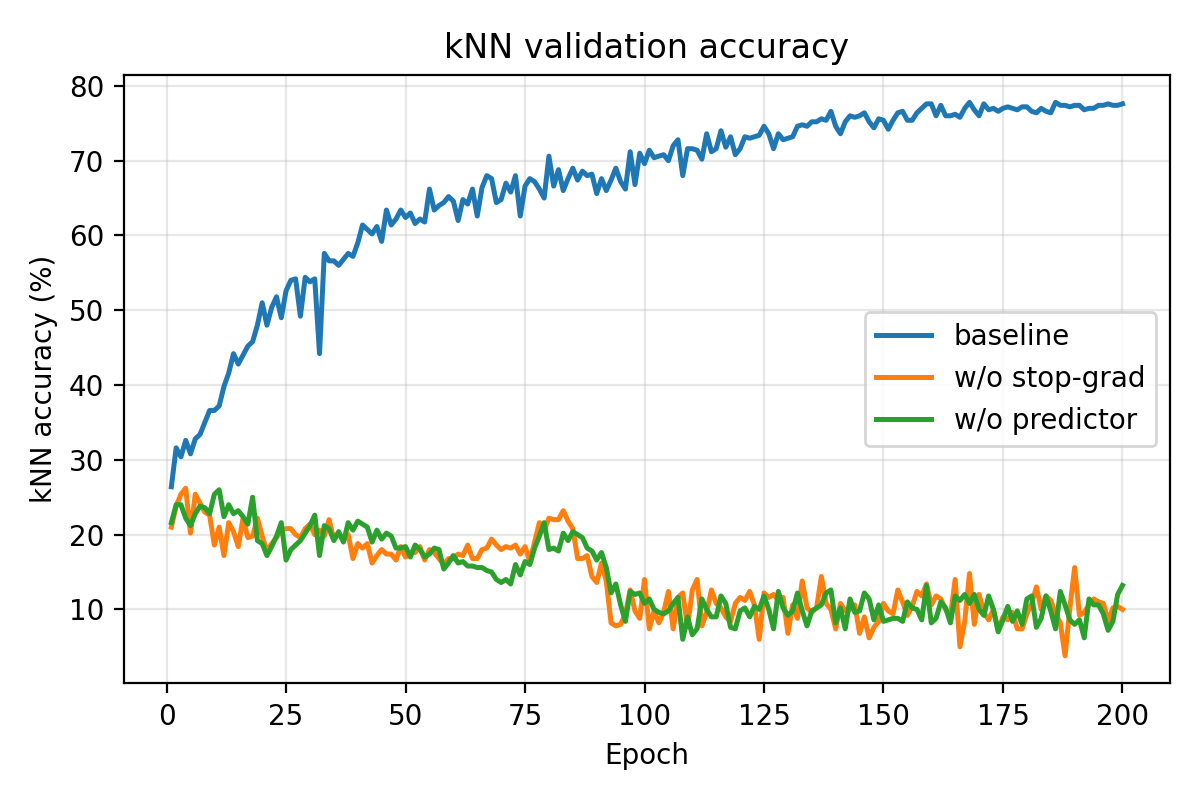
\includegraphics[width=0.325\linewidth]{figures/e200_arch_pretrain_knn.png}
\caption{Ablating the stop-gradient and the predictor (200 epochs): training loss, std of the $\ell_2$-normalized output (dashed: $1/\sqrt{d}$) and kNN accuracy. Both ablations collapse.}
\label{fig:arch}
\end{figure*}

\begin{table}[t]
\centering
\small
\setlength\tabcolsep{4pt}
\begin{tabular}{lcccc}
\toprule
Setting & Loss & Std & kNN & Lin.\ probe \\
\midrule
Baseline & $-0.908$ & 0.021 & 77.6 & 81.35 \\
no\_stopgrad & $-1.000$ & 0 & 10.0 & 10.00 \\
no\_predictor & $-1.000$ & 0 & 13.2$^*$ & 10.00 \\
\bottomrule
\end{tabular}
\caption{Architecture ablations, 200 epochs (final-epoch values; one unseeded run each, so the baseline differs from \cref{tab:aug}). $^*$Tie-breaking on identical features.}
\label{tab:arch}
\end{table}

Both variants reproduce the collapse reported in the original paper (\cref{fig:arch}, \cref{tab:arch}).
Within a few epochs the loss reaches its minimum of $-1$ and the output std drops toward 0, so every image is mapped to the same vector.
After 200 epochs the linear probe scores \emph{exactly} 10.00\% with training loss $\ln 10 = 2.303$, which is chance level for 10 classes. The original paper's 0.1\% is the same result for ImageNet's 1000 classes.

The two curves nearly coincide, as the paper predicts: without a predictor the gradient of \cref{eq:loss} has the direction of that of $\mathcal{D}(z_1,z_2)$, so the stop-gradient is in effect removed too, in line with DirectPred~\cite{tian2021directpred}. As in the paper we use one run per variant; an outcome of exactly chance leaves little room for seed variance.

\subsection{Ablation: Augmentation}
\label{sec:exp_aug}

\begin{table}[t]
\centering
\small
\setlength\tabcolsep{3pt}
\begin{tabular}{lcccc}
\toprule
Setting & Loss & kNN & Lin.\ probe & BN probe \\
\midrule
Baseline & $-0.909$ & 78.1 & \textbf{80.98}\pmstd{0.35} & \textbf{81.40}\pmstd{1.20} \\
no\_color & $-0.958$ & 44.9 & 50.36\pmstd{1.17} & 52.28\pmstd{1.25} \\
no\_crop & $-0.995$ & 19.3 & 17.50\pmstd{2.19} & 24.78\pmstd{1.54} \\
\bottomrule
\end{tabular}
\caption{Augmentation ablation, 200 epochs, mean (\pmstd{std}) over 3 pretraining seeds. Loss and kNN are final-epoch values averaged over seeds.}
\label{tab:aug}
\end{table}

\begin{figure*}[t]
\centering
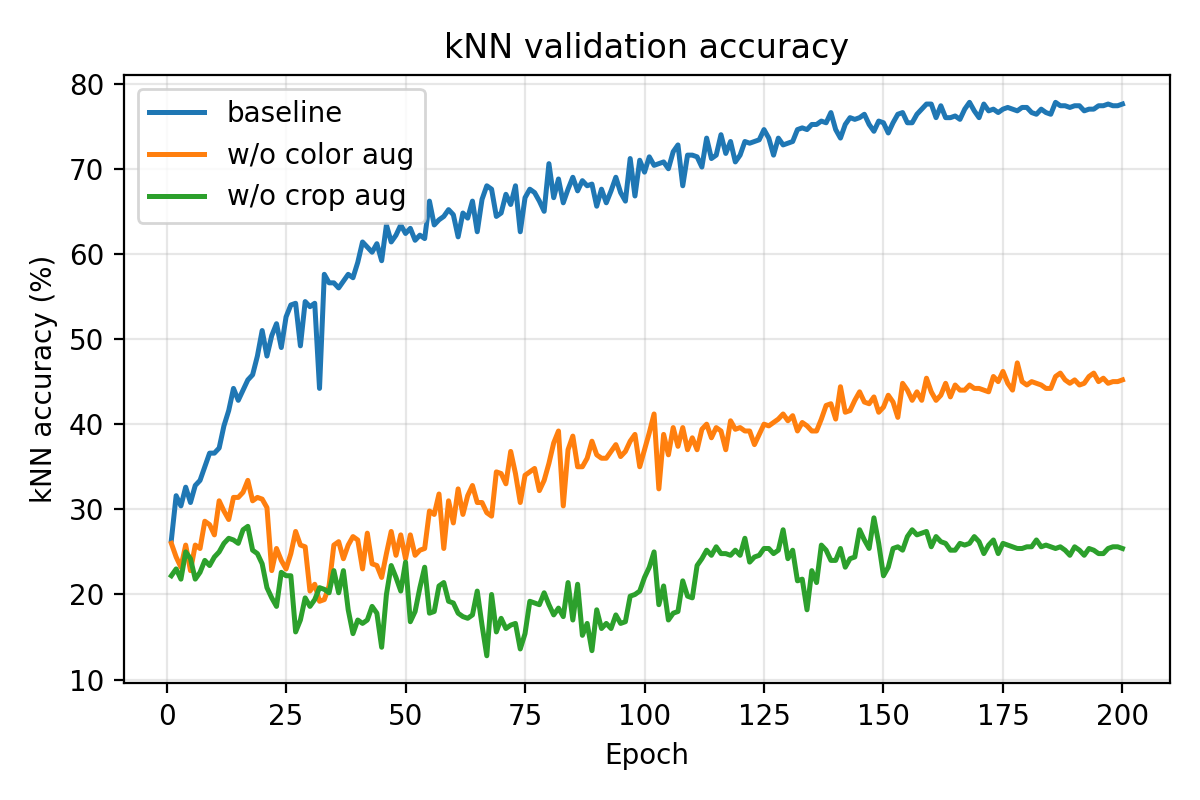
\includegraphics[width=0.31\linewidth]{figures/e200_aug_pretrain_knn.png}\hfill
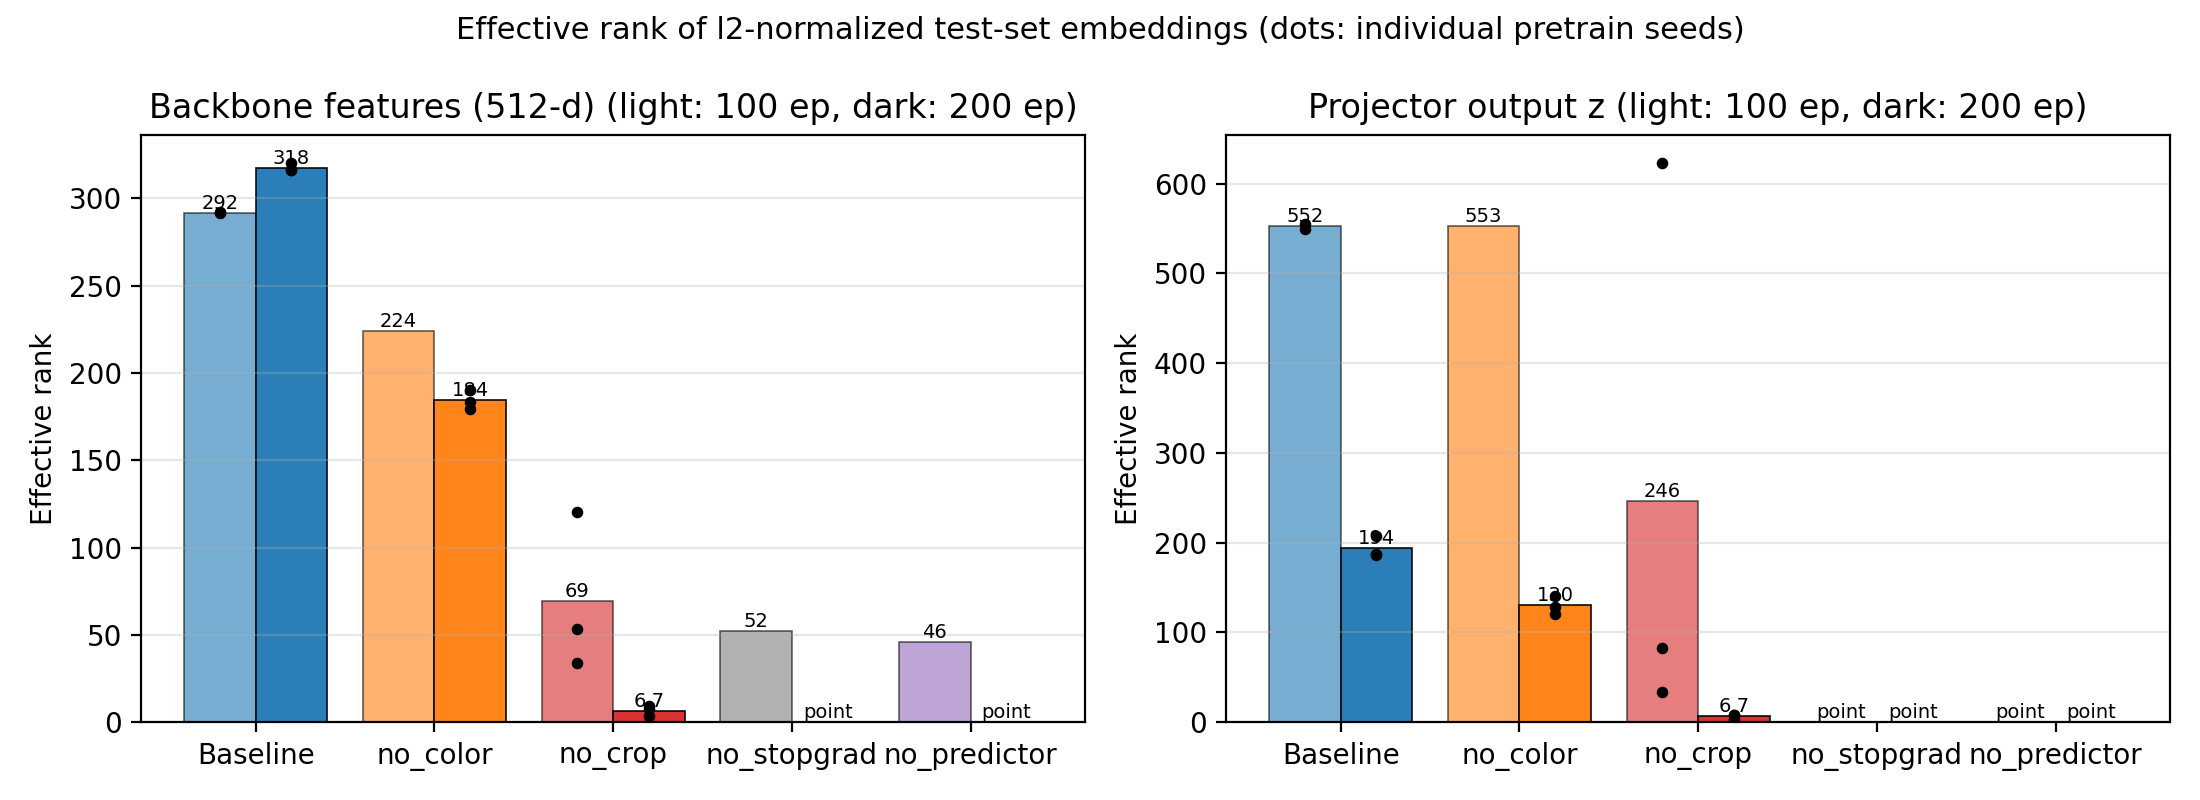
\includegraphics[width=0.67\linewidth]{figures/rank_bars.png}
\caption{Left: kNN accuracy during augmentation-ablation pretraining (one unseeded 200-epoch run each). Right: erank of test-set backbone features and projector output $z$ after 100 (light) and 200 (dark) epochs; bars: means, dots: seeds (100-ep baseline, no\_color unseeded). ``point'': all images map to one point (relative variance $<10^{-4}$).}
\label{fig:aug}
\end{figure*}

\paragraph{Lower loss, worse representation.}
Both variants reach a \emph{lower} loss than the baseline, because the views are easier to align, yet their accuracy is far lower (\cref{tab:aug}).
Under the BN probe (the standard one fails on no\_crop, below), removing color costs 29.1 points and removing crop 56.6 (81.4, 52.3, 24.8; $n{=}3$ each, all pairs $p_\text{Holm}<10^{-3}$); the standard probe gives the same order.
Cropping is therefore the more important augmentation, as for SimCLR~\cite{chen2020simclr}. BYOL~\cite{grill2020byol}, also without negatives, was \emph{less} sensitive than SimCLR, so we do not compare drop sizes across papers.

\paragraph{The standard probe fails on no\_crop.}
With lr 30, the linear probe on no\_crop's tiny-variance features never gets below training loss $\ln 10$, even with 200 epochs.
The BN probe standardizes them (validation picks lr 1.0, vs.\ 0.03 for the baseline) and raises no\_crop to 24.78\% ($+7.27$, paired $p{=}0.003$), still 57 points below the baseline under the same probe; we use it for no\_crop below.

\paragraph{no\_crop gets worse with more training.}
no\_color improves from 100 to 200 epochs ($43.9\rightarrow50.4$), but no\_crop moves the other way.
With 3 seeded 100-epoch runs and the BN probe, its accuracy drops from $38.17\pm2.39$ to $24.78\pm1.54$ (Welch $t{=}8.18$, df 3.4, $p{=}0.0023$; 95\% CI of the change $[-18.3,-8.5]$).
The 100- and 200-epoch models come from separate cosine schedules, but the decline also shows \emph{within} each 200-epoch run: no\_crop's kNN accuracy peaks at 27--33\% around epochs 15--21 and ends at 15--21\%, while the baseline's keeps rising (\cref{fig:aug}, left).

\paragraph{Dimensional collapse, not complete collapse.}
The effective rank explains these results (\cref{fig:aug}, right).
The 200-epoch no\_stopgrad and no\_predictor models are single points: their feature variance relative to the mean squared norm is $10^{-15}$ or smaller.
no\_crop is different. Its projector output $z$ still spreads out (relative variance 0.93, nonzero std), but occupies only about 4--8 of 2048 dimensions, and its backbone erank is just $6.7\pm2.8$, versus $317.5\pm2.4$ for the baseline.
This is \emph{dimensional collapse}~\cite{jing2022dimensional}.
It worsens with training: for every seed the backbone erank drops from 100 to 200 epochs (mean $69\rightarrow6.7$) together with the accuracy.
Without crops, \cref{eq:em} is nearly satisfied by \emph{any} color-invariant encoder, so the objective itself does not favor low rank; we hypothesize that weight decay removes directions the weak view difference no longer supports, as in DirectPred's eigenvalue dynamics~\cite{tian2021directpred}. Li \etal~\cite{li2022collapse} also report partial dimensional collapse in SimSiam.
\textbf{Stop-gradient and the predictor prevent complete collapse, but not dimensional collapse.}

It is not overfitting: loss and erank on unseen images match the training images.
All $t$-tests above stay significant after Holm correction under accuracy and F1 ($p_\text{Holm}\le0.017$), and under AUROC except the BN probe's gain over the standard probe ($p_\text{Holm}{=}0.11$; others $\le0.043$).

\subsection{What Does the Crop Contribute?}
\label{sec:exp_crop}


\Cref{tab:crop} reports the variants of \cref{sec:method} (200 epochs). Of the no\_crop$\to$baseline gap under the BN probe, masking recovers 68\%, crop\_in\_place 42\%, zoom\_out 21\% and the two shuffles 19--21\%. Backbone erank separates working from collapsed variants but not the middle (crop\_in\_place and zoom\_out: erank 75 vs.\ 74, 12 points apart).
Every adjacent pair among baseline, mask, crop\_in\_place, zoom\_out and no\_crop differs significantly (Welch over pretraining seeds, $p_\text{Holm}\le0.014$; accuracy and F1).

\begin{table}[t]
\centering
\small
\setlength\tabcolsep{3pt}
\begin{tabular}{lcccc}
\toprule
Variant & $n$ & erank & BN probe & AUROC \\
\midrule
Crop (baseline) & 3 & 318 & \textbf{81.40}\pmstd{1.20} & 97.80 \\
mask & 3 & 156 & 63.11\pmstd{0.53} & 93.82 \\
crop\_in\_place & 3 & 75 & 48.66\pmstd{1.68} & 88.31 \\
zoom\_out & 3 & 74 & 36.58\pmstd{2.09} & 81.88 \\
shuffle & 1 & 19 & 36.54 & 82.45 \\
shuffle\_shared & 1 & 11 & 35.27 & 81.75 \\
same\_crop & 3 & 5.5 & 27.65\pmstd{5.33} & 77.81 \\
No crop & 3 & 6.7 & 24.78\pmstd{1.54} & 72.33 \\
\bottomrule
\end{tabular}
\caption{Replacing RandomResizedCrop (200 epochs). Mean (\pmstd{std}) over $n$ pretraining seeds of the BN probe accuracy (each seed averaged over 5 finetuning seeds); erank is the backbone's; AUROC is macro one-vs-rest.}
\label{tab:crop}
\end{table}

\paragraph{The views must differ, not just the data.}
same\_crop sees as many distinct crops as the baseline, yet it is as poor as no\_crop ($27.7\pm5.3$ vs.\ $24.8\pm1.5$, $p{=}0.45$; same loss and kNN accuracy), so data diversity does not explain the failure: the two views must differ in \emph{which content} they show.

\paragraph{Partial content and rescaling are complementary.}
Hiding content (crop\_in\_place) helps more than rescaling (zoom\_out), and their sum (63\%) falls well short of the full crop. A two-way OLS on the 12 models gives an interaction of $+20.9$ points (95\% CI 16.5--25.4, $p_\text{Holm}\le2\!\times\!10^{-4}$, accuracy and F1; additive in AUROC, which saturates near 98). Two confounds limit this: the crop \emph{enlarges} a part while zoom\_out \emph{shrinks} the whole, and only the single-factor cells contain mean-filled regions.
Scattered masking is the best single replacement ($+14.5$ over crop\_in\_place at equal visible area, $p_\text{Holm}{=}0.014$), possibly because views hide different parts of the object, as InfoMin~\cite{tian2020infomin} suggests and MSN~\cite{assran2022msn} exploits.

\paragraph{Each model learns mainly the invariance its views demand.}
To see why masking trails the crop by 18 points, we retrieve each of 2,000 test images from a transformed copy by nearest neighbor in backbone space (3 seeds).
The crop model finds 94.8\% of $2\times$ zoomed-in copies but 3.4\% of 50\%-masked ones; the mask model is the reverse (0.7\% vs.\ 99.7\%, though this test resembles its training views), zoom\_out finds only zoomed-out copies (100\%), crop\_in\_place 46.8\% of masked ones, and no\_crop $\le$2.1\% of any.
Masking never requires matching a part to the whole at another scale, which, judging by the probe, matters most for recognition (cf.~\cite{purushwalkam2020demystifying}; three transforms only).

\paragraph{A different layout is not a useful difference.}
shuffle and its control shuffle\_shared end level (36.5 vs.\ 35.3), although a fixed encoder (the 1000-epoch baseline) finds shuffled views \emph{less} similar (cosine 0.82) than crops (0.90); we hypothesize that a CNN with global pooling matches tiles from local statistics. Beyond near-identical views (cosine 0.98: no\_crop, same\_crop), view dissimilarity does not predict quality.


%-------------------------------------------------------------------------
\section{Limitations}
\label{sec:limitations}

(i) Neither erank nor std ranks settings: no\_color's erank falls from 100 to 200 epochs ($224\to184$) as accuracy rises, and the 1000-epoch baseline's std halves while its erank (392) and accuracy are highest. (ii) The crop decomposition lacks an enlarge-without-occlusion cell. (iii) With $n{=}3$ seeds the Welch df is only 2--4. (iv) The shuffles have one seed and same\_crop's seeds span 22--33 points, which test-set McNemar tests~\cite{mcnemar1947} ignore. Mean-filled regions, the shared mask grid and tile seams may act as shortcuts.
(v) The tuned SFT's best lr (0.3) lies at the grid edge, so the 25.3-point gap is an upper bound; we did not fine-tune end to end. (vi) Only ResNet-18 at $96^2$; baseline seed 123 was resumed at epoch 25 without its RNG state.

%-------------------------------------------------------------------------
\section{Conclusion}
\label{sec:conclusion}
With 1,000 labels, SimSiam features beat a tuned from-scratch network by 25 points; without stop-gradient or predictor they collapse completely.
Without cropping, the loss is lower and the std nonzero, yet features collapse onto a few dimensions and degrade with training, which erank and a properly scaled probe detect.
The views must differ in content: a shared crop is as harmful as none, and each model becomes invariant mainly to what its views vary, of which the crop's part-to-whole rescaling serves recognition best.

%%%%%%%%% REFERENCES
{
    \small
    \bibliographystyle{ieeenat_fullname}
    \bibliography{main}
}

\end{document}
